\documentclass[12pt]{article}
\usepackage{Sweave}
\usepackage{myVignette}
\usepackage[authoryear,round]{natbib}
\bibliographystyle{plainnat}
\DefineVerbatimEnvironment{Sinput}{Verbatim}
{formatcom={\vspace{-2.5ex}},fontshape=sl,
  fontfamily=courier,fontseries=b, fontsize=\scriptsize}
\DefineVerbatimEnvironment{Soutput}{Verbatim}
{formatcom={\vspace{-2.5ex}},fontfamily=courier,fontseries=b,%
  fontsize=\scriptsize}
%%\VignetteIndexEntry{Implementation Details}
%%\VignetteDepends{Matrix}
%%\VignetteDepends{lme4}
\begin{document}


\setkeys{Gin}{width=\textwidth}
\title{Linear mixed model implementation in lme4}
\author{Douglas Bates\\Department of Statistics\\University of
  Wisconsin -- Madison\\\email{Bates@wisc.edu}}
\maketitle
\begin{abstract}
  Expressions for the evaluation of the profiled log-likelihood or
  profiled log-restricted-likelihood of a linear mixed model, the
  gradients and Hessians of these criteria, and update steps for an
  ECME algorithm to optimize these criteria are given in Bates and
  DebRoy (2004).  A representation of linear mixed models using
  positive semidefinite symmetric matrices and dense matrices is given
  in Bates (2004).  In this paper we present details of that
  representation and those computational methods in the \code{lme4}
  package for R.
\end{abstract}

\begin{Schunk}
\begin{Soutput}
Loading required package: Matrix 
Loading required package: latticeExtra 
\end{Soutput}
\end{Schunk}
\section{Introduction}
\label{sec:Intro}

General formulae for the evaluation of the profiled log-likelihood and
profiled log-restricted-likelihood in a linear mixed model are given
in \citet{bate:debr:2004} and the use of a sparse matrix
representation for such models is described in \citet{bate:2004}.  The
purpose of this paper is to describe the details of the implementation
of this representation and those computational methods in the \code{lme4}
package for \RR{}.

Because we concentrate on the computational methods and the
representation, the order and style of presentation will be based on
the sequence of calculations, not on the sequence in which the results
would be derived.  We will emphasize ``what'' and not ``why''.  For
the ``why'', refer to the papers cited above.

In \S\ref{sec:Form} we describe the form and representation of the
model.  The calculation of the criteria to be optimized by the
parameter estimates and related quantities is discussed in
\S\ref{sec:Cholesky}.  Details of the calculation of the ECME step and the
evaluation of the gradients of the criteria are given in
\S\ref{sec:ECME} and those of the Hessian in \S\ref{sec:Hessian}.  In
\S\ref{sec:Unconstrained} we give the details of an unconstrained
parameterization for the model and the transformation of our
results to this parameterization.

\section{Form and representation of the model}
\label{sec:Form}

We consider linear mixed models of the form
\begin{equation}
  \label{eq:lmeGeneral}
  \by=\bX\bbeta+\bZ\bb+\beps\quad
  \beps\sim\mathcal{N}(\bzer,\sigma^2\bI),
  \bb\sim\mathcal{N}(\bzer,\sigma^2\bOmega^{-1}),
  \beps\perp\bb
\end{equation}
where $\by$ is the $n$-dimensional response vector, $\bX$ is an
$n\times p$ model matrix for the $p$ dimensional fixed-effects vector
$\bbeta$, $\bZ$ is the $n\times q$ model matrix for the
$q$ dimensional random-effects vector $\bb$ that has a Gaussian
distribution with mean $\bzer$ and relative precision matrix $\bOmega$
(i.e., $\bOmega$ is the precision of $\bb$ relative to the precision
of $\beps$), and $\beps$ is the random noise assumed to have a
spherical Gaussian distribution.  The symbol $\perp$ indicates
independence of random variables.  The matrix $\bX$ has full
column rank and $\bOmega$ is positive definite.

The random effects vector $\bb$ and the columns of $\bZ$ are divided
into $k$ outer blocks associated with grouping factors $\bff_i,
i=1,\dots,k$ in the data.  Because so many of the expressions that we
will use involve the grouping factors and quantities associated with
them, we will reserve the letter $i$ to index the grouping factors and
related quantities. We will not explicitly state the range of $i$,
which will always be $i=1,\dots,k$.

The outer blocks in $\bb$ and the columns of $\bZ$ are further
subdivided into $m_i$ inner blocks of size $q_i$ where $m_i$ is the
number of levels of $\bff_i$ (i.e.{} the number of distinct values in
$\bff_i$). Each grouping factor has associated with it an $n\times
q_i$ model matrix $\bZ_i$.  The full model matrix $\bZ$ is derived
from the grouping factors $\bff_i$ and these submodel matrices
$\bZ_i$.

Random effects in different outer blocks are independent.  Within each
of these blocks, the inner blocks of random effects are independent
and identically distributed with mean $\bzer$ and $q_i\times q_i$
variance-covariance matrix $\sigma^2\bOmega_i\inv$.  Thus $\bOmega$ is
block diagonal in $k$ blocks of size $m_i q_i\times m_i q_i$ and each
of these blocks is itself block diagonal in $m_i$ blocks, each of
which is the positive definite symmetric $q_i\times q_i$ matrix
$\bOmega_i$.  We call this a \emph{repeated block/block diagonal}
matrix.

\subsection{Model specification and representation}
\label{sec:Representation}

Like most model fitting functions in the S language, the \code{lme}
function in the \code{lme4} package uses a formula/data specification.
The formula specifies how to evaluate the response $\by$ and the
fixed-effects model matrix $\bX$ in the data frame provided as the
\code{data} argument.  An additional argument named \code{random}
specifies the names of the grouping factors and the formulae for
evaluation of the model matrices $\bZ_i$.

Standard optional arguments, such as \code{na.action} and
\code{subset}, are passed through to the \code{model.frame} function
that returns the model frame in which to evaluate all the formulae of
the model.  The \code{drop.unused.levels} optional argument is set to
\code{TRUE} so that unused levels in any factors are dropped during
creation of the model frame.  Thus there is no ambiguitiy regarding
the number of levels $m_i$ of each of the $\bff_i$.  Every level in
each of the $\bff_i$ must occur at least once in the model frame.

\subsubsection{Pairwise crosstabulation}

We begin by ordering the grouping factors so that $m_1\ge m_2\ge \dots
\ge m_k$ and, if $k>1$, forming their \emph{pairwise crosstabulation}.
This is the crossproduct matrix, $\bT=\tilde{\bZ}\trans\tilde{\bZ}$,
for the \emph{variance components model} determined by these grouping
factors.  (In a variance components model $q_1=q_2=\dots=q_k=1$ and
each of the $\tilde{\bZ}_i$ is the $n\times 1$ matrix of $1$s.  The
$i$th outer block of columns in $\tilde{\bZ}$ is the set of indicator
columns for the levels of $\bff_i$.  The name ``variance components''
reflects the fact that, in this model, each of the $\bOmega_i$, which
are scalars, is the relative precision of the component of the
variation in the response attributed to factor $\bff_i$.)

In fact it is not necessary to form and store $\bT$.  All that we need
are the locations of the nonzeros in the off-diagonal blocks of the
representation
\begin{equation}
  \label{eq:PairwiseCrosstab}
  \bT=\begin{bmatrix}
    \bT_{(1,1)}&\bT_{(2,1)}\trans&\dots&\bT_{(k,1)}\trans\\
    \bT_{(2,1)}&\bT_{(2,2)}&\dots&\bT_{(k,2)}\trans\\
    \vdots&\vdots&\ddots&\vdots\\
    \bT_{(k,1)}&\bT_{(k,2)}&\dots&\bT_{(k,k)}\trans
  \end{bmatrix} .
\end{equation}
(Because the $i$th outer block of columns in $\tilde{\bZ}$ is a set of
indicators, the diagonal blocks will themselves be diagonal and their
patterns of nonzeros are trivial.)  The blocks in the strict lower
triangle, $\bT_{(i,j)}, i>j$ are stored as a list of compressed,
sparse, column-oriented matrices (see Appendix~\ref{app:Sparse} for
details).  Only the column pointers and the row indices of these
sparse matrices are used..

These off-diagonal blocks are easily calculated because the integer
representations of the factors $\bff_i$ and $\bff_j$ form the row and
column indices in a (possibly redundant) triplet representation of
$\bT_{(i,j)}$.  All that we need to do is convert the triplet
representation to the compressed, sparse, column-oriented
representation.  This common conversion is easily accomplished with
standard software.

We check whether each of the matrices $\bT_{(j,j-1)},j=2,\dots,k$ has
exactly one nonzero in each column.  If so, the grouping factors form
a \emph{nested sequence} in that each level of factor $\bff_i$ occurs
with exactly one level of factor $\bff_j, i<j\le k$.  In the
compressed, sparse, column-oriented format it is easy to determine the
number of nonzeros in each column because these are the successive
differences in the column pointers.

If the grouping factors form a nested sequence (and a single grouping
factor is trivially a nested sequence) there is no need for further
symbolic analysis.  If not, which is to say that we have multiple,
non-nested grouping factors, we continue the symbolic analysis for the
unit lower triangular factor $\tL$ in the LDL form of the Cholesky
decomposition of $\bT$~\citep{Davis:2004}.

This symbolic analysis is performed on rows of blocks in the lower
triangle of $\tL$, where the blocks of $\tL$ correspond to those
of $\bT$
\begin{equation}
  \label{eq:blockwiseL}
  \tL=\begin{bmatrix}
    \bI&\bzer&\dots&\bzer\\
    \tL_{(2,1)}&\tL_{(2,2)}&\dots&\bzer\\
    \vdots&\vdots&\ddots&\vdots\\
    \tL_{(k,1)}&\tL_{(k,2)}&\dots&\tL_{(k,k)}
  \end{bmatrix} .
\end{equation}
We emphasize that we are only determining the positions of the
nonzeros in the blocks of $\tL$, not performing an actual
decomposition.  (The decomposition would fail for $k>1$ because $\bT$
is only positive semidefinite, not positive definite.  It is composed
of multiple blocks of indicators and the row sums within each block
are always unity.)

Because $\bT_{(1,1)}$ is diagonal, the block in the $(1,1)$ position
of $\tL$ will be both diagonal and unit, which is to say that it is
the identity matrix of size $m_1$.  A consequence of the $(1,1)$ block
being the identity is that the structure of the first column of blocks
of $\tL$ is the same as the corresponding block of $\bT$.  That is,
the nonzeros in $\tL_{(j,1)}$ are in the same positions as those in
$\bT_{(j,1)}$ for $1<j\le k$.

The off-diagonal nonzero positions in $\tL_{(2,2)}$ are determined
from the union of the off-diagonal nonzeros positions in
$\bT_{(2,2)}$, of which there are none, and those in
$\tL_{(2,1)}\tL_{(2,1)}\trans=\bT_{(2,1)}\bT_{(2,1)}\trans$.  The
number of nonzeros in $\tL_{(2,2)}$ can be changed by permuting the
levels of $\bff_2$, which causes a permutation of the rows of the
blocks $\bT_{(2,i)}$ and the columns of the blocks $\bT_{(i,2)}$.  We
determine a fill-reducing permutation of the levels of $\bff_2$ using
routines from the Metis~\citep{Metis} graph-partitioning package
applied to the incidence graph of $\bT_{(2,1)}\bT_{(2,1)}\trans$.
(This is the graph of $m_2$ nodes in which nodes $s$ and $t$ are
connected by an edge if and only if
$\left\{\bT_{(2,1)}\bT_{(2,1)}\trans\right\}_{s,t}$ is nonzero.)  We
apply this permutation to the columns of all blocks $\bT_{(i,2)}$ and
the rows of all blocks $\bT_{(2,i)}$.

The symbolic analysis function from the LDL package applied to
$\bT_{(2,1)}\bT_{(2,1)}\trans$ (after permuting the rows of
$\bT_{(2,1)}$) provides the positions of the nonzeros in
$\tL_{(2,2)}$, from which we determine the positions of the nonzeros
in $\tL_{(2,2)}\inv$.  The positions of the nonzeros in $\tL_{(3,2)}$
are those of $\bT_{(3,2)}\tL_{(2,2)}\inv$.  The next step in the
iteration is to form the union of the nonzero positions of
$\tL_{(3,2)}\tL_{(3,2)}\trans$ and the nonzero positions in
$\bT_{(3,1)}\bT_{(3,1)}\trans$ from which we determine a fill-reducing
permutation for the levels of $\bff_3$.  The process is continued
until a fill-reducing permutation for the levels of $\bff_k$ and the
structure of $\tL_{(k,k)}$ and $\tL_{(k,k)}\inv$ are determined.

As part of the symbolic analysis of each diagonal block, the
elimination tree~\citep{Davis:2004} of the block is determined and
stored as an integer array of length $m_i$.  It is straightforward to
check the number of terminal nodes in this tree.  If the elmination
tree for $\tL_{(i,i)}$ is found to have only one terminal node then
$\tL_{(i,i)}\inv$ will be dense. Furthermore, all subsequent diagonal
blocks will be dense so there is no purpose in checking for a
fill-reducing permutation of the levels of $\bff_j,i<j\le k$, and the
symbolic analysis can be terminated.

\subsubsection{Allocating storage}

In the numeric representation of the model we will write the augmented
model matrix of size $n\times(p+1)$ obtained by appending $\by$ to
$\bX$ as $\tilde{\bX}=\left[\bX,\by\right]$.  We can allocate the
storage for the sparse matrix representation of the model using the
results of the symbolic analysis and the numbers of columns in the
model matrices, $q_i,i=1,\dots,k$ and $(p+1)$.

We will store $\bOmega$, $\bZ\trans\bZ$, $\bZ\trans\tilde{\bX}$,
$\tilde{\bX}\trans\tilde{\bX}$ and components $\RZZ$, $\tRZX$ and $\tRXX$ of
the Cholesky decomposition
\begin{equation}
  \label{eq:tildeCrossProdGen}
  \begin{bmatrix}
    \bZ\trans\bZ+\bOmega & \bZ\trans\tilde{\bX} \\
    \tilde{\bX}\trans\bZ & \tilde{\bX}\trans\tilde{\bX}
  \end{bmatrix}=\bR\trans\bR\quad\text{where}\quad\bR=
  \begin{bmatrix}
    \RZZ & \tRZX\\
    \bzer& \tRXX
  \end{bmatrix} .
\end{equation}
in one of four possible formats: as a dense matrix, as a block/block
sparse matrix, as a block/block diagonal matrix, or as a repeated
block/block diagonal matrix.

For example, we have already indicated that $\bOmega$ is repeated
block/block diagonal so we store it in the \code{Omega} slot as a list
of $k$ symmetric matrices of sizes $q_i\times q_i$ (only the upper
triangles of the symmetric matrices are used).

The matrices $\bZ\trans\tilde{\bX}$ and
$\tilde{\bX}\trans\tilde{\bX}$, and the decomposition components
$\tRZX$, and $\tRXX$ matrices are stored as dense matrices in slots
named \code{ZtX}, \code{XtX}, \code{RZX} and \code{RXX}, respectively.

The matrix $\bZ\trans\bZ$ is stored in a symmetric, sparse
column-oriented format like that of $\bT$ in
(\ref{eq:PairwiseCrosstab}) except that $\bZ\trans\bZ$ has both inner
and outer blocks.  The $k\times k$ grid of outer blocks
$(\bZ\trans\bZ)_{(i,j)}$ is determined by the grouping factors.  These
outer blocks correspond to the blocks $\bT_{(i,j)}$ in $\bT$.  The
diagonal outer block $(\bZ\trans\bZ)_{(i,i)}$ is itself block diagonal
in $m_i$ blocks of size $q_i\times q_i$.  We store the upper triangles
of these inner blocks in an array of size $q_i\times q_i\times m_i$.
Block $(\bZ\trans\bZ)_{(i,j)}$ for $j<i\le k$ is subdivided into inner
blocks of size $q_i\times q_j$ corresponding to the levels of grouping
factors $i$ and $j$.  Because an inner block of
$(\bZ\trans\bZ)_{(i,j)}$ is nonzero if and only if the corresponding
element of $\bT_{(i,j)}$ is nonzero, we can use the column pointers
and row indices from $\bT_{(i,j)}$ for $(\bZ\trans\bZ)_{(i,j)}$ with
the convention that they index the inner blocks, not the individual
elements, of $(\bZ\trans\bZ)_{(i,j)}$.  The inner blocks are stored in
a dense array of dimension $q_i\times q_j\times n_{(i,j)}$ where
$n_{(i,j)}$ is the number of nonzeros in $\bT_{(i,j)}$.  This is the
block/block sparse matrix format.

Instead of calculating $\RZZ$ we calculate the LDL form
\begin{equation}
  \label{eq:bigLDL}
  \bZ\trans\bZ+\bOmega=\bL\bD\bL\trans
\end{equation}
where $\bL$ is block/block unit lower triangular (i.e.{} block/block lower
triangular with all the inner diagonal blocks in the $i$th outer
diagonal block being the $q_i\times q_i$ identity matrix) and $\bD$ is
block/block diagonal.

Just as the column pointers and row indices of the blocks of $\bT$ can
be used for the outer blocks of $\bZ\trans\bZ$, we can use the column
pointers and row indices of $\tL$, which we have determined in the
symbolic analysis, for the outer blocks of
\begin{equation}
  \label{eq:Lform}
  \bL=
  \begin{bmatrix}
    \bI & \bzer & \dots & \bzer\\
    \bL_{(2,1)} & \bL_{(2,2)} & \dots & \bzer\\
    \vdots    & \vdots & & \bzer\\
    \bL_{(k,1)} & \bL_{(k,2)} & \dots & \bL_{(k,k)}
  \end{bmatrix} .
\end{equation}
That is, the same structure as $\tL_{(i,j)}$
applies to the blocks $\bL_{(i,i)}, 1<i\le k$, $\bL_{(i,i)}, 1<i\le k$,
and $\bL_{(i,j)}, 1\le j<i\le k$ except that each nonzero in
$\tL_{(i.j)}$ corresponds to a block of size $q_i\times q_j$ in
$\bL_{(i.j)}$.

From the symbolic analysis we also have the column pointers and row
indices for $\tL^{-1}_{(i,i)}$, corresponding to the diagonal outer
blocks of $\bL^{-1}$.  We allocate storage for these diagonal outer
blocks only.  Note that $\bL^{-1}$ is block/block unit lower
triangular just like $\bL$.  Because the inner diagonal blocks of
these matrices are always the identity, these inner blocks are not
explicitly stored.  Neither $\bL_{(1,1)}=\bI$ nor
$\left(\bL^{-1}\right)_{(1,1)}=\bI$ require any storage to be
allocated.

We have used fill-reducing permutations of the levels of the grouping
factors $\bff_j,j=2,\dots,k$.  These can decrease, sometimes
dramatically, the amount of storage required for the $\tL_{(i,i)}$ but
generally they do not result in compact storage of
$\tL_{(i,i)}^{-1}$.  In the worst case the matrix $\tL_{(2,2)}^{-1}$
will be dense or nearly dense, resulting in a storage requirement of
approximately $q_2^2 m_2(m_2+1)/2$ elements for the array holding the
numeric values for the $(2,2)$ outer block of $\bL^{-1}$.

The matrix $\bD$ is block/block diagonal. It is stored as a list of
$k$ arrays of sizes $q_i\times q_i\times m_i$.

After allocating the storage we evaluate $\by$, $\bX$ and the $\bZ_i$
then update the contents of the \code{XtX}, \code{ZtX}, and \code{ZtZ}
slots.  We allocate the storage and update the contents of the storage
in separate steps so we can update the numeric values without
reallocating storage during iterative algorithms for fitting
generalized linear mixed models or nonlinear mixed models.

\section{Evaluation of the objective}
\label{sec:Cholesky}

If prior estimates of the $\bOmega_i$ are available, we set the
\code{Omega} slot accordingly.  Otherwise we form initial estimates
from the matrices $\bZ_i$, as described in
\citet[ch.~3]{pinh:bate:2000}.  We then begin iterative optimization
of the estimation criterion with respect to the $\bOmega_i$ or with
respect to the unconstrained parameter $\btheta$ that determines the
$\bOmega_i$, as described in \S\ref{sec:Unconstrained}.

In this section we will describe the steps in evaluating the objective
function (i.e.{} the function to be optimized w.r.t.{} the $\bOmega_i$
or w.r.t.{} $\btheta$) given the current values of the $\bOmega_i$.
Recall that after setting values of the $\bOmega_i$ we form the
Cholesky decomposition (\ref{eq:tildeCrossProdGen})
\begin{equation*}
  \begin{bmatrix}
    \bZ\trans\bZ+\bOmega & \bZ\trans\tilde{\bX} \\
    \tilde{\bX}\trans\bZ & \tilde{\bX}\trans\tilde{\bX}
  \end{bmatrix}=\bR\trans\bR\quad\text{where}\quad\bR=
  \begin{bmatrix}
    \RZZ & \tRZX\\
    \bzer& \tRXX
  \end{bmatrix} .
\end{equation*}
and $\tilde{\bX}$ incorporates both $\bX$ and $\by$.  In some cases
it will be convenient to consider $\bX$ and $\by$ separately and we will
write the components of the Cholesky decomposition as if they were
\begin{equation}
  \label{eq:CrossProdGen}
  \begin{bmatrix}
    \bZ\trans\bZ+\bOmega & \bZ\trans\bX  & \bZ\trans\by \\
    \bX\trans\bZ         & \bX\trans\bX  & \bX\trans\by \\
    \by\trans\bZ         & \by\trans\bX  & \by\trans\by
  \end{bmatrix}=\bR\trans\bR\quad\text{where}\quad\bR=
  \begin{bmatrix}
    \RZZ & \RZX & \rZy \\
    \bzer    & \RXX & \rXy \\
    \bzer    & \bzer    & \ryy
  \end{bmatrix}
\end{equation}
even though they are stored in the form of (\ref{eq:tildeCrossProdGen}).

Recall also that $\RZZ$ is calculated and stored in the LDL form.
Instead of storing the symmetric positive definite inner blocks of the
block/block diagonal $\bD$, we calculate and store their upper
Cholesky factors.  We write the block/block diagonal matrix of upper
Cholesky factors as $\bD^{1/2}$ and its transpose as
$\bD^{\mathsf{T}/2}$.  (Note that transposing a block/block diagonal
matrix only requires transposing the inner blocks.)  The quantity
$\log\left|\bD\right|$ is evaluated as the sum of the logarithms of
the squares of the diagonal elements of the inner diagonal blocks of
$\bD^{1/2}$.

The next step in the factorization is to solve for $\tRZX$ in
\begin{equation}
  \label{eq:RZX}
  \RZZ\trans\tRZX=\bL\bD^{\mathsf{T}/2}\tRZX=\bZ\trans\tilde{\bX}
\end{equation}
using blocked sparse matrix techniques (see
Appendix~\ref{app:blocked}), storing the result in the \code{RZX}
slot.  Finally, dense matrix operations are used to downdate the
densely stored $\tilde{\bX}\trans\tilde{\bX}$ and obtain the upper
Cholesky factor $\tRXX$ that satisfies
\begin{equation}
  \label{eq:RXX}
  \tRXX\trans\tRXX=
  \tilde{\bX}\trans\tilde{\bX}-\tRZX\trans\tRZX ,
\end{equation}
and provides $\log\left(\left|\RXX\right|^2\right)$ and $\ryy$.

The \code{status} slot is a pair of logical values called
\code{factored} and \code{inverted}.  It is set to \code{(TRUE,
  FALSE)} indicating that the factorization is current and that it has
not been inverted.

In a separate calculation the logarithm of the determinant
\begin{equation}
  \label{eq:OmegaDet}
  \log |\bOmega|=\sum_{i=1}^k m_i \log |\bOmega_i|
\end{equation}
is evaluated from the Cholesky factors of the $\bOmega_i$.  The
function to be minimized w.r.t.{} $\btheta$, called the \emph{profiled
  deviance}, is
\begin{equation}
  \label{eq:ProfiledLogLik}
  f(\btheta)=\log\left|\bD\right|-\log\left|\bOmega\right|
  + n\left[1+\log\left(\frac{2\pi\ryy^2}{n}\right)\right]
\end{equation}
for ML estimation or
\begin{equation}
  \label{eq:ProfiledLogRestLik}
  f_R(\btheta)=
  \log\left|\bD\right|+\log\left(\left|\RXX\right|^2\right)
  - \log\left|\bOmega\right|
  + (n-p)\left[1+\log\left(\frac{2\pi\ryy^2}{n-p}\right)\right]
\end{equation}
for REML.

\subsection{Inverting the factorization}
\label{ssec:Inverting}

Evaluatation of the objective function does not require inversion of
the factorization nor does evaluation of many other quantities of
interest, such as the conditional variance estimates
$\widehat{\sigma^2}=\ryy^2/n$ and $\widehat{\sigma}_R^2=\ryy^2/(n-p)$,
the conditional fixed effects estimates, $\widehat{\bbeta}$, which satisfy
$\RXX\widehat{\bbeta}=\rXy$, 
and the conditional modes of
the random effects, $\widehat{\bb}$, which satisfy
\begin{equation}
  \label{eq:bbhat}
  \bD^{1/2}\bL\trans\widehat{\bb}=\rZy-\RZX\widehat{\bbeta}
\end{equation}

However, if we wish to evaluate the ECME step or the gradient and/or
the Hessian of the objective, it is convenient to invert some parts of
the decomposition.  We invert the dense upper triangular matrix
$\tRXX$ in place, producing $\RXX^{-1}$ in the first $p$ rows and
columns, $1/\ryy$ in the $(p+1,p+1)$ position, and
$-\widehat{\bbeta}/\ryy$ in the first $p$ rows of the $p+1$st column.
We also invert each of the triangular inner blocks of $\bD^{1/2}$ in
place producing $\bD^{-1/2}$.  The inverses of the outer blocks on the
diagonal of $\bL$ are also determined and stored separately.  (In
general the diagonal outer blocks cannot be inverted in place.  The
number of nonzero inner blocks in the inverse of an outer block on the
diagonal can be different from the number of nonzero inner blocks in
the outer diagonal block itself.)  Notice that this last operation
is trivial in the case of a single grouping factor or multiple, nested
grouping factors because all the outer diagonal blocks in $\bL$ are
identity matrices.

The matrix $\tRZX{\tRXX}^{-1}$ is evaluated as a dense matrix product
then each column of
$-\bL\invtrans\bD^{-1/2}\left(\tRZX{\tRXX}^{-1}\right)$ is evaluated
using blocked sparse matrix operations (see Appendix~\ref{app:blocked}
for details) and stored in the \code{RZX} slot.  The first $p$ columns
of the result, which are $-\bL\invtrans\bD^{-1/2}\RZX\RXX^{-1}$, are
used to create products involving the matrix $\vb$, which is the
unscaled, conditional, REML variance-covariance of the random effects
\begin{equation}
  \label{eq:VbDef}
  \begin{aligned}
    \vb&= \begin{bmatrix}\bI&\bzer\end{bmatrix}
    \left(
      \begin{bmatrix}\RZZ\trans & \bzer \\ \RZX\trans & \RXX\trans\end{bmatrix}
      \begin{bmatrix}\RZZ & \RZX \\ \bzer & \RXX\end{bmatrix}
    \right)^{-1}
    \begin{bmatrix} \bI\\\bzer \end{bmatrix}\\
    &= \begin{bmatrix}\bI&\bzer\end{bmatrix}
    \begin{bmatrix}\RZZ\inv&-\RZZ\inv\RZX\RXX\inv\\\bzer&\RXX\inv\end{bmatrix}
    \begin{bmatrix}\RZZ\invtrans&\bzer\\
      -\RXX\invtrans\RZX\trans\RZZ\invtrans&\RXX\invtrans\end{bmatrix}
    \begin{bmatrix} \bI\\\bzer \end{bmatrix}\\
    &=\begin{bmatrix}\RZZ\inv&-\RZZ\inv\RZX\RXX\inv\end{bmatrix}    
    \begin{bmatrix}\RZZ\invtrans\\
      -\RXX\invtrans\RZX\trans\RZZ\invtrans\end{bmatrix}\\
    &=\RZZ\inv\RZZ\invtrans
    +\RZZ\inv\RZX\RXX\inv\RXX\invtrans\RZX\trans\RZZ\invtrans\\
    &=\left(\bZ\trans\bZ+\bOmega\right)\inv
    +\RZZ\inv\RZX\RXX\inv\RXX\invtrans\RZX\trans\RZZ\invtrans\\
    &=\left(\bZ\trans\bZ+\bOmega\right)\inv
    +\bL\invtrans\bD^{-1/2}\RZX\RXX\inv
    \RXX\invtrans\RZX\trans\bD^{-\mathsf{T}/2}\bL\inv\\
  \end{aligned}
\end{equation}
The $p+1$st column is $-\widehat{\bb}/\ryy$.

The \code{status} flag is changed to \code{(TRUE, TRUE)} indicating
that the factorization is current and that it is the inverted
components that are stored in the \code{RZX}, \code{RXX}, and
\code{Dfac} slots and that the \code{LIx} slot if current.


\section{Examples}
\label{sec:Examples}

To illustrate this representation and these operations we consider
some examples of common types of mixed effects models.

\subsection{Single grouping factor}
\label{sec:SingleGrouping}

The \code{Early} data set in the \code{lme4} package is from a
longitudinal study on an early childhood intervention program.  These
data are described in \citet[ch.~3]{Sing:Will:2003}.  The response is
a cognitive development score, \code{cog}, measured at ages 1, 1.5,
and 2 years (\code{age}) on 103 infants (identified by \code{id}); 58
of whom were in the treatment group and 45 in the control group
(identified by \code{trt}).  We convert the \code{age} measurement to
``time on study'', \code{tos} as the treatment began at age 0.5 years.
\begin{Schunk}
\begin{Sinput}
> data(Early)
> Early$tos <- Early$age - 0.5
> str(Early)
\end{Sinput}
\begin{Soutput}
`data.frame':	309 obs. of  5 variables:
 $ id : Factor w/ 103 levels "86","87","77",..: 12 12 12 17 17 17 22 22 22 8 ...
 $ cog: int  103 119 96 106 107 96 112 86 73 100 ...
 $ age: num  1 1.5 2 1 1.5 2 1 1.5 2 1 ...
 $ trt: Factor w/ 2 levels "N","Y": 2 2 2 2 2 2 2 2 2 2 ...
 $ tos: num  0.5 1 1.5 0.5 1 1.5 0.5 1 1.5 0.5 ...
\end{Soutput}
\end{Schunk}
A lattice plot of the longitudinal scores is given in Figure~\ref{fig:EarlyData}.
\begin{figure}[tbp]
  \centering
  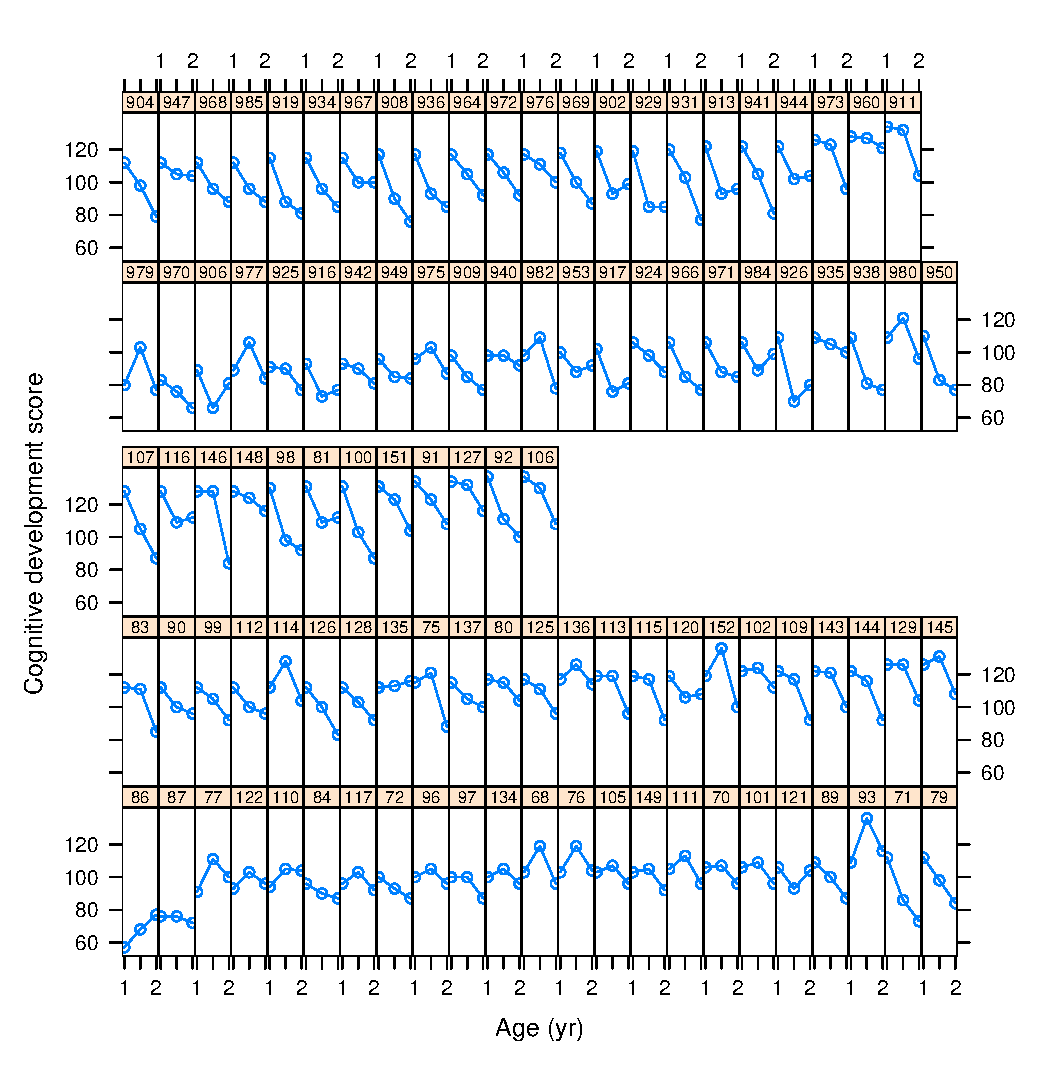
\includegraphics[width=\textwidth]{figs/Example-EarlyData}
  \caption[Cognitive development scores]{Cognitive development scores
    for 103 infants; 45 in the control group (identification numbers
    above 900) and 58 in the treatment group. The data from 
    each infant are displayed in separate panels. Those for the
    infants in the treatment group are in the lower three rows of
    panels; the control group are in the upper two rows.  Within each
    group the panels are ordered by increasing initial cognitive
    score.}
  \label{fig:EarlyData}
\end{figure}

These data are grouped by subject, as is common in longitudinal data.
The only grouping factor for random effects is \code{id}.  (The
subjects are themselves grouped into a treatment group and a control
group but that dichotomy would be modeled with fixed effects, not
random effects.)  As an initial model an analyst may fit an
\emph{unconditional growth} model~\cite[ch.~4]{Sing:Will:2003}
\begin{Schunk}
\begin{Sinput}
> fm1 <- lmer(cog ~ tos + (tos | id), Early)
\end{Sinput}
\end{Schunk}
or proceed immediately to a model that allows for the effects of the
treatment 
\begin{Schunk}
\begin{Sinput}
> fm2 <- lmer(cog ~ tos * trt + (tos | id), Early)
\end{Sinput}
\end{Schunk}

The structure of the resulting object is
\begin{Schunk}
\begin{Sinput}
> str(fm2)
\end{Sinput}
\begin{Soutput}
Formal class 'lmer' [package "lme4"] with 21 slots
  ..@ flist   :List of 1
  .. ..$ id: Factor w/ 103 levels "86","87","77",..: 12 12 12 17 17 17 22 22 22 8 ...
  ..@ perm    :List of 1
  .. ..$ id: int [1:103] 0 1 2 3 4 5 6 7 8 9 ...
  ..@ Parent  :List of 1
  .. ..$ id:List of 2
  .. .. ..$ index: int [1:103] -1 -1 -1 -1 -1 -1 -1 -1 -1 -1 ...
  .. .. ..$ block: int [1:103] -1 -1 -1 -1 -1 -1 -1 -1 -1 -1 ...
  ..@ D       :List of 1
  .. ..$ id: num [1:2, 1:2, 1:103]  0.502  0.000 -0.639  0.526  0.502 ...
  ..@ bVar    :List of 1
  .. ..$ id: num [1:2, 1:2, 1:103]  0.661  0.000 -0.336  0.277  0.661 ...
  ..@ L       :List of 1
  .. ..$ :Formal class 'cscBlocked' [package "Matrix"] with 3 slots
  .. .. .. ..@ p: int [1:104] 0 0 0 0 0 0 0 0 0 0 ...
  .. .. .. ..@ i: int(0) 
  .. .. .. ..@ x: num[1:2, 1:2, 0 ] 
  ..@ ZZpO    :List of 1
  .. ..$ id:Formal class 'cscBlocked' [package "Matrix"] with 3 slots
  .. .. .. ..@ p: int [1:104] 0 1 2 3 4 5 6 7 8 9 ...
  .. .. .. ..@ i: int [1:103] 0 1 2 3 4 5 6 7 8 9 ...
  .. .. .. ..@ x: num [1:2, 1:2, 1:103] 3.96 0.00 4.82 9.48 3.96 ...
  ..@ Omega   :List of 1
  .. ..$ id: num [1:2, 1:2] 1.00e+10 0.00e+00 3.97e+10 1.58e+11
  ..@ REML    : logi TRUE
  ..@ RXX     : num [1:5, 1:5] 0.126 0.000 0.000 0.000 0.000 ...
  ..@ RZX     : num [1:206, 1:5] -0.1226  0.0225 -0.1226  0.0225 -0.1226 ...
  ..@ XtX     : num [1:5, 1:5] 309   0   0   0   0 ...
  ..@ ZtZ     :List of 1
  .. ..$ :Formal class 'cscBlocked' [package "Matrix"] with 3 slots
  .. .. .. ..@ p: int [1:104] 0 1 2 3 4 5 6 7 8 9 ...
  .. .. .. ..@ i: int [1:103] 0 1 2 3 4 5 6 7 8 9 ...
  .. .. .. ..@ x: num [1:2, 1:2, 1:103] 3 0 3 3.5 3 0 3 3.5 3 0 ...
  ..@ ZtX     : num [1:206, 1:5] 3 3 3 3 3 3 3 3 3 3 ...
  ..@ cnames  :List of 2
  .. ..$ id    : chr [1:2] "(Intercept)" "tos"
  .. ..$ .fixed: chr [1:5] "(Intercept)" "tos" "trtY" "tos:trtY" ...
  ..@ devComp : num [1:4] 274.28  92.37  13.01   9.98
  ..@ deviance: Named num [1:2] 2371 2360
  .. ..- attr(*, "names")= chr [1:2] "ML" "REML"
  ..@ nc      : int [1:3] 2 5 309
  ..@ Gp      : int [1:2] 0 206
  ..@ status  : Named logi [1:2] FALSE FALSE
  .. ..- attr(*, "names")= chr [1:2] "factored" "inverted"
  ..@ call    : language lmer(formula = cog ~ tos * trt + (tos | id), data = Early)
\end{Soutput}
\end{Schunk}

\section{Frechet derivatives}
\label{sec:Frechet}

We will denote the Frechet derivative of the matrix $\bOmega$ with
respect to $\bOmega_i$ by $\der_{\bOmega_i}\bOmega$.  This is a four
dimensional array that can be regarded as an indexed set of $q_i^2$
matrices, each the same size as $\bOmega$.  These matrices, which we
call the $q_i^2$ ``faces'' of the array, are indexed by the rows $r$
and the columns $c$, $r,c=1,\dots,q_i$ of $\bOmega_i$.  The $(r,c)$th
face, which we write as $\der_{i:r,c}\bOmega$, is the derivative of
$\bOmega$ with respect to the $(r,c)$th element of $\bOmega_i$. It is
a repeated block/block diagonal matrix where all of the outer diagonal
blocks are zero except for the $(i,i)$ diagonal block which is block
diagonal in $m_i$ blocks of $\bbe_r\bbe_c\trans$, where $\bbe_j$ is
the $j$th column of the identity matrix of size $q_i$.

An expression of the form
$\tr\left[\left(\der_{\bOmega_i}\bOmega\right)\bM\right]$ where $\bM$
is a matrix of the same size as $\bOmega$ evaluates to $q_i^2$ scalars
indexed by $r$ and $c$, $r,c=1,\dots,q_i$, which we convert to a
$q_i\times q_i$ matrix in the obvious way.  This type of expression
can be simplified as
\begin{equation}
  \label{eq:derOmegai}
  \tr\left[(\der_{\bOmega_i}\bOmega)\bM\right]
  = \sum_{j=1}^{m_i}\tr\left[(\der_{\bOmega_i}\bOmega_i)\bM_{i,i,j,j}\right]
  = \sum_{j=1}^{m_i}\bM_{i,i,j,j}\trans
\end{equation}
where $\bM_{i,i,j,j}$ is the $j$th inner diagonal block in the $i$th
outer diagonal block of $\bM$.  To establish the last equality in
(\ref{eq:derOmegai}) note that for any $q_i\times q_i$ matrix $\bA$
the entry in row $r$ and column $c$ of
$\tr\left[(\der_{\bOmega_i}\bOmega_i)\bA\right]$ is
\begin{equation}
  \label{eq:rowRcolCentry}
  \left\{\tr\left[(\der_{\bOmega_i}\bOmega_i)\bA\right]\right\}_{r,c}
  = \tr\left[\bbe_r\bbe_c\trans\bA\right]
  = \tr\left[\bbe_c\trans\bA\bbe_r\right]
  = \bbe_c\trans\bA\bbe_r
  = \bA_{c,r}
\end{equation}
If $\bM$ is symmetric, as is the case in all the expressions of this
form that we consider, then
$\tr\left[\left(\der_{\bOmega_i}\bOmega\right)\bM\right]$ will be
symmetric.

Expressions of this form that we will require include 
\begin{equation}
  \label{eq:derOmegaInv}
  \begin{aligned}
  \tr\left[\left(\der_{\bOmega_i}\bOmega\right)\left(\bOmega\right)^{-1}\right]
    &= \sum_{j=1}^{m_i}\left(\bOmega_{i,i,j,j}\right)\inv\\
    &= m_i\bOmega_i\inv
  \end{aligned},
\end{equation}
\begin{equation}
  \label{eq:bbDer}
  \tr\left[\left(\der_{\bOmega_i}\bOmega\right) \left(
      \frac{\widehat{\bb}}{\ryy} \frac{\widehat{\bb}}
      {\ryy} \trans\right)\right] = \bB_i \bB_i\trans
\end{equation}
where $\bB_i$ is the $q_i\times m_i$ matrix whose $j$ column is
$\widehat{\bb}_{i,j}/\ryy, j=1,\dots,m_i$ (recall that these vectors
are in the $p+1$st column of the \code{RZX} slot after the inversion
step), and $\tr \left[ \left( \der_{\bOmega_i} \bOmega \right)
  (\bZ\trans\bZ+\bOmega)^{-1} \right]$.

The last term requires evaluation of the
inner diagonal blocks of 
\begin{equation}
  \label{eq:ZtZinv}
  \left(\bZ\trans\bZ +\bOmega\right)^{-1}=\left(\RZZ\trans\RZZ\right)\inv=
  =\bL\invtrans\bD^{-1/2}\bD^{-\mathsf{T}/2}\bL^{-1}
\end{equation}
When $k=1$, $\bL$ is an identity
matrix and the result is simply
\begin{equation*}
  \tr\left[\left(\der_{\bOmega_i}\bOmega\right)
    \bD^{-1/2}\bD^{-\mathsf{T}/2}\right]=
  \sum_{j=1}^{m_1}\bD_{1:j}^{-1/2}\bD_{1:j}^{-\mathsf{T}/2} .
\end{equation*}
When $k>1$ we must evaluate the crossproduct of each of the $m_i$
inner blocks of $q_i$ columns in the $i$th outer block of columns of
$\bD^{-\mathsf{T}/2}\bL^{-1}=\RZZ\invtrans$, which we do using blocked, sparse
matrix techniques.  See Appendix~\ref{ssec:InverseBlocks} for details.

For REML results we also need
\begin{multline}
  \label{eq:Vbterm}
  \tr\left[\left(\der_{\bOmega_i}\bOmega\right)\vb\right] = \\
  \tr\left[\left(\der_{\bOmega_i}\bOmega\right)
    \RZZ\inv\RZZ\invtrans\right]
  + \tr\left[\left(\der_{\bOmega_i}\bOmega\right)
    \RZZ\inv\RZX\RXX\inv\RXX\invtrans\RZX\trans\RZZ\invtrans\right]
\end{multline}
We have just described how to calculate the first term in
(\ref{eq:Vbterm}).  The second term is evaluated as the crossproducts
of the $m_i$ inner blocks of $q_i$ rows in the $i$th outer block of the rows
of $-\RZZ\inv\RZX\RXX\inv$, which is calculated and stored in the
\code{RZX} slot during the inversion of the factorization, as
described in \S\ref{ssec:Inverting}.

\section{ECME updates}
\label{sec:ECME}

ECME iterations provide a stable, but only linearly convergent,
optimization algorithm for the objective functions $f$ and $f_R$.  We
use a moderate number (the default is 20) of them to refine our
initial estimates $\bOmega_i^{(0)}$ and bring us into the region of
the optimum before switching to Newton iterations on the unconstrained
parameter vector $\btheta$.

The ECME iterations can be defined in terms of the $\bOmega_i$.  At
the $\nu$th iteration, $\bOmega^{(\nu+1)}$ is defined to be the
repeated block/block diagonal, symmetric, positive definite matrix
that satisfies the $k$ systems of equations
\begin{equation}
  \label{eq:theta1}
  \tr\left[\der_{\bOmega_i}\bOmega\left(
      \frac{\widehat{\bb}^{(\nu)}}{\widehat{\sigma}^{(\nu)}}
      \frac{\left.{\widehat{\bb}}^{(\nu)}\right.\trans}{\widehat{\sigma}^{(\nu)}}+
      \left(\bZ\trans\bZ+\bOmega^{(\nu)}\right)^{-1}
      -\left(\bOmega^{(\nu+1)}\right)^{-1}\right)\right]=\bzer
\end{equation}
for ML estimates or the $k$ systems
\begin{equation}
  \label{eq:theta1R}
  \tr\left[\der_{\bOmega_i}\bOmega\left(
      \frac{\widehat{\bb}^{(\nu)}}{\widehat{\sigma}_R^{(\nu)}}
      \frac{\left.{\widehat{\bb}}^{(\nu)}\right.\trans}{\widehat{\sigma}_R^{(\nu)}}+
      \vb^{(\nu)}
      -{\bOmega^{(\nu+1)}}^{-1}\right)\right]=\bzer
\end{equation}
for REML.

The results of \S\ref{sec:Frechet} provide
\begin{equation}
  \label{eq:theta1soln}
  \bOmega_i^{(\nu+1)}=m_i\left\{
    \tr \left[ \left( \der_{\bOmega_i} \bOmega \right)
      (\bZ\trans\bZ+\bOmega^{(\nu)})^{-1}
    \right]+n\bB_i^{(\nu)}{\bB_i^{(\nu)}}\trans\right\}^{-1}
\end{equation}
for ML and
\begin{equation}
  \label{eq:theta1Rsoln}
  \bOmega_i^{(\nu+1)}=m_i\left\{
    \tr \left[ \left( \der_{\bOmega_i} \bOmega \right)\vb
    \right]+(n-p)\bB_i^{(\nu)}{\bB_i^{(\nu)}}\trans\right\}^{-1} 
\end{equation}
for REML.
\subsection{Gradient evaluations}
\label{ssec:Gradient}

The gradients of (\ref{eq:ProfiledLogLik}) and (\ref{eq:ProfiledLogRestLik})
with respect to $\bOmega_i$ are
\begin{align}
  \label{eq:gradDev}
  \nabla_{\bOmega_i}f&=\tr\left[\der_{\bOmega_i}\bOmega\left(
      (\bZ\trans\bZ+\bOmega)^{-1}-\bOmega^{-1}+
      \frac{\widehat{\bb}}{\widehat{\sigma}}
      \frac{\widehat{\bb}}{\widehat{\sigma}}\trans\right)\right]\\
  \label{eq:gradDevRest}
  \nabla_{\bOmega_i} f_R&=\tr\left[\der_{\bOmega_i}\bOmega\left(
      \vb-\bOmega^{-1}+
      \frac{\widehat{\bb}}{\widehat{\sigma}_R}
      \frac{\widehat{\bb}}{\widehat{\sigma}_R}\trans\right)\right]
\end{align}
and we have already described how to calculate all those terms.

\section{Evaluation of the Hessian}
\label{sec:Hessian}

The Hessians of the scalar functions $f$ and $f_R$ are symmetric
matrices of second derivatives.  As for the calculation of the
gradient, we first evaluate the Hessian with respect to the
$Q=\sum_{i=1}^k q_i^2$ dimensional vector
$\bomega=\left[\bomega_1\trans,\dots,\bomega_k\trans\right]\trans$
where $\bomega_i=\ovec\bOmega_i$ and `$\ovec$' is the vectorization
function that produces a column vector from a matrix by concatenating
the columns.  That is, we temporarily ignore the fact that the
$\bOmega_i$ must be positive definite and symmetric and we consider each of the
elements in these matrices separately.  In \S\ref{sec:Unconstrained}
we describe an unconstrained parameter vector $\btheta$ of length
$\sum_{i=1}^k\binom{q_i+1}{2}$ and the conversion of the gradient and
Hessian for $\bomega$ to the corresponding quantities for $\btheta$.

For convenience we index the $Q$ elements of $\bomega$ by triplets
$i:r,c$ denoting the element at row $r$ and column $c$ of
$\bOmega_i$.  \citet{bate:debr:2004} show that the element in row
$i:r,c$ and column $j:s,t$ of the Hessian is
\begin{equation}
  \label{eq:HessianML}
  \begin{aligned}
    \left\{\nabla_{\bomega}^2 f\right\}_{i:r,c;j:s,t}=
    &\tr\left[\der_{i:r,c}\left(\der_{j:s,t}\bOmega\right)
      \left(\left(\bZ\trans\bZ+\bOmega\right)\inv-\bOmega\inv+
        \frac{\widehat{\bb}}{\widehat{\sigma}}
        \frac{{\widehat{\bb}}\trans}{\widehat{\sigma}}\right)\right]\\
    &-\tr\left[\der_{i;r,c}\bOmega\left(\bZ\trans\bZ+\bOmega\right)\inv
      \der_{j;s,t}\bOmega\left(\bZ\trans\bZ+\bOmega\right)\inv\right]\\
    &+\tr\left[\left(\der_{i;r,c}\bOmega\right)\bOmega\inv
      \left(\der_{j;s,t}\bOmega\right)\bOmega\inv\right]\\
    &-2\frac{{\widehat{\bb}}\trans}{\widehat{\sigma}}
    \left(\der_{i;r,c}\bOmega\right)\vb
    \left(\der_{j;s,t}\bOmega\right)\frac{\widehat{\bb}}{\widehat{\sigma}}\\
    &-\frac{1}{n}
    \left(\frac{{\widehat{\bb}}\trans}{\widehat{\sigma}}
      \left(\der_{i;r,c}\bOmega\right)
      \frac{\widehat{\bb}}{\widehat{\sigma}}\right)
    \left(\frac{{\widehat{\bb}}\trans}{\widehat{\sigma}}
      \left(\der_{j;s,t}\bOmega\right)
      \frac{\widehat{\bb}}{\widehat{\sigma}}\right)
  \end{aligned}
\end{equation}
for ML estimates, and
\begin{equation}
  \label{eq:HessianREML}
  \begin{aligned}
    \left\{\nabla_{\bomega}^2 f_R\right\}_{i:r,c;j:s,t}=
    &\tr\left[\der_{i:r,c}\left(\der_{j:s,t}\bOmega\right)
      \left(\vb-\bOmega\inv+
        \frac{\widehat{\bb}}{\widehat{\sigma}}
        \frac{{\widehat{\bb}}\trans}{\widehat{\sigma}}\right)\right]\\
    &-\tr\left[\der_{i;r,c}\bOmega\vb
      \der_{j;s,t}\bOmega\vb\right]\\
    &+\tr\left[\left(\der_{i;r,c}\bOmega\right)\bOmega\inv
      \left(\der_{j;s,t}\bOmega\right)\bOmega\inv\right]\\
    &-2\frac{{\widehat{\bb}}\trans}{\widehat{\sigma}_R}
    \left(\der_{i;r,c}\bOmega\right)\vb
    \left(\der_{j;s,t}\bOmega\right)\frac{\widehat{\bb}}{\widehat{\sigma}_R}\\
    &-\frac{1}{n}
    \left(\frac{{\widehat{\bb}}\trans}{\widehat{\sigma}_R}
      \left(\der_{i;r,c}\bOmega\right)
      \frac{\widehat{\bb}}{\widehat{\sigma}_R}\right)
    \left(\frac{{\widehat{\bb}}\trans}{\widehat{\sigma}_R}
      \left(\der_{j;s,t}\bOmega\right)
      \frac{\widehat{\bb}}{\widehat{\sigma}_R}\right)
  \end{aligned}
\end{equation}
for REML.

The matrix $\der_{j:s,t}\bOmega$ is constant so the first term in both
(\ref{eq:HessianML}) and (\ref{eq:HessianREML}) is zero.

\section{Unconstrained parameterization}
\label{sec:Unconstrained}

The vector
$\btheta=\left[\btheta_1\trans,\dots,\btheta_k\trans\right]\trans$ is
an unconstrained parameterization of $\bOmega$ based on the LDL form
of the Cholesky decomposition of the $\bOmega_i$
\begin{equation}
  \label{eq:OmegaLDL}
  \bOmega_i=\bL_i\bD_i\bL_i\trans .
\end{equation}
where $\bL_i$ is a $q_i\times q_i$ unit lower triangular matrix and
$\bD_i$ is a $q_i\times q_i$ diagonal matrix with positive diagonal
elements.  We use the $q_i$ logarithms of the diagonal elements of
$\bD_i$, written $\bdelta_i$, and, when $q_i>1$, the row-wise
concatenation of the $\binom{q_i}{2}$ elements in the strict lower
triangle of $\bL_i$, written $\blambda_i$, as the $\binom{q+1}{2}$
dimensional unconstrained parameter
$\btheta_i=\left[\bdelta_i\trans,\blambda_i\trans\right]\trans$


Let $g$ be any scalar function of the $\bOmega_i$ such that the
$q_i\times q_i$ gradient matrices $\nabla_{\bdelta_i}f$ are symmetric.
(Both $f$, the objective for ML estimation, and $f_R$, the objective
for REML estimation, are such functions.)  The components
$\nabla_{\bdelta_i}g$ and $\nabla_{\blambda_i}g$ of the gradient
vector $\nabla_{\btheta_i}g$ can be evaluated from the symmetric
gradient matrix $\nabla_{\bOmega_i}g$ and the
derivative of the product (\ref{eq:OmegaLDL}).  For example,
\begin{equation}
  \label{eq:deltaPartial}
  \begin{aligned}
    \left\{\nabla_{\bdelta_i}g\right\}_j
    &=\tr\left[\left(\nabla_{\bOmega_i}g\right)
      \frac{\partial \bOmega_i}{\partial \left\{\bdelta_i\right\}_j}\right]\\
    &=\tr\left[\left(\nabla_{\bOmega_i}g\right)\bL_i\frac{\partial{\bD_i}}
      {\partial\left\{\bdelta_i\right\}_j}\bL_i\trans\right]\\
    &=\exp{\left\{\bdelta_i\right\}_j}\bbe_j\trans
    \bL_i\left(\nabla_{\bOmega_i}g\right)\trans\bL_i\bbe_j\\
    &=\left\{\bR_i\left(\nabla_{\bOmega_i}g\right)\bR_i\trans\right\}_{j,j}
  \end{aligned}
\end{equation}
for $j=1,\dots,q_i$, where $\bR_i$ is the upper Cholesky factor of $\bOmega_i$.
The partial derivative with respect to
element $t$ of $\blambda_i$, which determines the $r,c$th element of
$\bL_i$, is
\begin{equation}
  \label{eq:lambdaPartial}
  \begin{aligned}
    \left\{\nabla_{\blambda_i}g\right\}_t
    &=\tr\left[\left(\nabla_{\bOmega_i}g\right)
      \frac{\partial\bOmega_i}{\partial\left\{\blambda_i\right\}_t}\right]\\
    &=\tr\left[\left(\nabla_{\bOmega_i}g\right)
      \bbe_r\bbe_c\trans\bD_i\bL_i\trans
      +\left(\nabla_{\bOmega_i}g\right) 
      \bL_i\bD_i\bbe_c\bbe_r\trans\right]\\
    &=\bbe_c\trans\bD_i\bL_i\trans\left(\nabla_{\bOmega_i}g\right)\bbe_r
    +\bbe_r\trans\left(\nabla_{\bOmega_i}g\right)\bL_i\bD_i\bbe_c\\
    &=2\left\{\left(\nabla_{\bOmega_i}g\right)\bL_i\bD_i\right\}_{c,r}\\
    &=2\left\{\left(\nabla_{\bOmega_i}g\right)\bR_i\trans\bD_i^{1/2}\right\}_{c,r}
  \end{aligned}
\end{equation}

\section{Acknowledgements}
\label{sec:Ack}

This work was supported by U.S.{} Army Medical Research and Materiel
Command under Contract No.{} DAMD17-02-C-0119.  The views, opinions
and/or findings contained in this report are those of the authors and
should not be construed as an official Department of the Army
position, policy or decision unless so designated by other
documentation.

\appendix

\section{Sparse matrix formats}
\label{app:Sparse}

The basic form of sparse matrix storage, called the \emph{triplet}
form, represents the matrix as three arrays of length \code{nz}, which
is the number of nonredundant nonzero elements in the matrix.  The
\code{i} array contains the row indices, the \code{j} array the column
indices, and the \code{x} array the values of the nonzero elements.  A
\emph{column-oriented} triplet form requires that the elements of
these arrays be such that \code{j} is nondecreasing.  A sorted,
column-oriented triplet form is such that elements in \code{i}
corresponding to the same \code{j} index are in increasing order. That
is, the arrays are ordered by column and, within column, by row.

In column-oriented storage, multiple elements in the same column
produce runs in \code{j}.  A \emph{compressed}, column-oriented
storage form replaces \code{j} by \code{p}, an array of pointers to
the indices (in \code{i} and \code{x}) of the first element in each
column.  If there are $n$ columns in the matrix, this array is of
length $n+1$, with the last element of \code{p} being one greater than
the index of last element in the last column.  Then the differences of
successive elements of \code{p} give the number of nonzeros in each
column.

In the implementation in the \code{Matrix} package for R, the indices
\code{i}, \code{j}, and \code{p} are \code{0}-based, as in the C
language, (i.e.{} the first element of an array has index \code{0})
not \code{1}-based, as in the S language.  Thus the first element of
\code{p} is always zero.  
  

\section{Blocked sparse matrix operations}
\label{app:blocked}

We take advantage of the blocked sparse structure of $\bZ\trans\bZ$,
$\bOmega$, $\bL$ and $\bD$ in operations involving these matrices.
Consider, for example, the operation of solving for $\tRZX$ in the
system (\ref{eq:RZX}),
$\bL\bD^{\mathsf{T}/2}\tRZX=\bZ\trans\tilde{\bX}$.  Let $\bu$ be a
column of $\bD^{\mathsf{T}/2}\tRZX$ and $\bv$ be the corresponding
column of $\bZ\trans\tilde{\bX}$.  The corresponding column of the
result, which is $\bD^{-\mathsf{T}/2}\bu$, is easily evaluated from
$\bu$. (Recall that $\bD^{-1/2}$ is block/block diagonal, i.e. block
diagonal in $k$ outer blocks of sizes $m_i q_i\times m_i q_i$ each of
which is itself block diagonal in $m_i$ blocks of size $q_i\times
q_i$, and that $\bD^{-1/2}$ is calculated and stored during the
inversion step.)  Both $\bu$ and $\bv$ can be divided into $k$ outer
blocks of sizes $m_i q_i$, which we denote $\bu_i$ and $\bv_i$, and
each of the outer blocks can be divided into $m_i$ inner blocks of
size $q_i$, which we denote $\bu_{i:j}$ and $\bv_{i:j}$.

Because $\bL$ is lower triangular, the blocks of $\bv$ can be
evaluated in a blockwise forward solve.  That is, the blocked
equations are solved in the order
\begin{equation}
  \label{eq:blockwiseForward}
  \begin{aligned}
    \bL_{(1,1)}\bu_1 &= \bv_1\quad\Longrightarrow\quad \bI\bu_1 =
    \bu_1 = \bv_1\\
    \bL_{(2,2)}\bu_2 &= \bv_2-\bL_{(2,1)}\bu_1\\
    &\vdots\\
    \bL_{(k,k)}\bu_k &= \bv_k-\bL_{(k,k-1)}\bu_{k-1}-\dots-\bL_{(k,1)}\bu_1
  \end{aligned}
\end{equation}
Notice that the solution in the first block does not require any
calculation because $\bL_{(1,1)}$ is always the identity.  In many
applications $k=1$ and the operation of solving for $\bL\bu=\bv$ can
be skipped entirely.  In most other applications the size of $\bu_1$
dominates the size of the other components so that being able to set
$\bu_1=\bv_1$ represents a tremendous savings in computational effort.

We take advantage of the blocked, sparse columns of the outer blocks
of $\bL$ in evaluations of the form $\bv_2-\bL_{(2,1)}\bu_{1}$.  That
is, we evaluate $\bL_{(2,1)}\bu_{1}$ using the blocks of size
$q_2\times q_1$ skipping blocks that we know will be zero as we update
the inner blocks of $\bu_2$ in place.  The solutions of systems of the
form $\bL_{(i,i)}\bu_i=\tilde{\bv}_i$ where $\tilde{\bv}_i$ is the
updated $\bv_i$ are also done in inner blocks taking advantage of the
sparsity of $\bL_{(i,i)}^{-1}$.  Recall that in the case of nested grouping
factors the $\bL_{(i,i)}$ are all identity matrices and this step is
skipped.


\subsection{Accumulating diagonal blocks of the inverse}
\label{ssec:InverseBlocks}

The ECME steps and the gradient evaluation require
\begin{equation}
  \label{eq:InverseBlocks}
    \tr\left[\der_{\bOmega_i}\bOmega\left(\bZ\trans\bZ+\bOmega\right)^{-1}\right]
    = \tr\left[\left(\der_{\bOmega_i}\bOmega\right)
      \left(\bD^{-\mathsf{T}/2}\bL\inv\right)\trans
      \left(\bD^{-\mathsf{T}/2}\bL\inv\right)\right]
\end{equation}
which will be the sum of the crossproducts of the $m_i$ inner blocks
of $q_i$ columns in the $i$th outer block of columns of
$\bD^{-\mathsf{T}/2}\bL\inv$.

When $i=k=1$ the result is
$\sum_{j=1}^{m_1}\bD^{-1/2}_{1:j}\bD^{-\mathsf{T}/2}_{1:j}$, which can
be evaluated in a single call to the level-3 BLAS routine
\code{dsyrk}.  (Having the 3 dimensional array containing the $m_i$
inner blocks of the $i$th outer block of $\bD^{-1/2}$ in the form that
allows this to be done in a single, level-3 BLAS call is the reason
that we store and invert the upper triangular factors of inner blocks
of $\bD$.)

When $i=1$ and $k>1$ we initialize the result from the $(1,1)$ block
as above, then add the crossproducts of inner blocks of columns in the
outer $(2,1)$ block, the outer $(3,1)$ block, and so on.  These blocks
of columns are calculated sparsely.  During the initial decomposition
we evaluate and store (in blocked, sparse format) $\bL^{-1}_{(i,i)}$
for $1<i\le k$.
  
\bibliography{lme4}
\end{document}


\section{Frechet derivatives}
\label{sec:Frechet}

In sections that follow we will use the symbol $\der$ for the Frechet
derivative.  When used with a vector subscript, such as in
$\der_{\theta_i}\bOmega$, it represents a three dimensional array
where each face is the same size as $\bOmega$ and the number of faces
is the number of elements in $\btheta_i$.  When used with a matrix
subscript, such as $\der_{\bOmega_i}\bOmega$ it represents a four
dimensional array.  When used without a subscript it indicates the
pattern that the expression will take when a specific subscript is
used.

In the gradient and ECME calculations the $\der$ symbol occurs in
expressions of the form
\begin{equation*}
  \tr\left[(\der\bOmega)(\bM)\right]
\end{equation*}
where $\tr$ denotes the trace operator and $\bM$ is an
$M\times M$ matrix ($M=\sum_{i=1}^k m_i q_i$).  If we use
a vector subscript on $\der$, the expression evaluates to a vector of the same length
as the subscript vector.  If we use a matrix subscript, it
evaluates to a matrix of the same dimensions as the subscript matrix.


Let us consider the specific example of
$\tr\left[\left(\der\bOmega\right)\bOmega^{-1}\right]$.
\begin{equation}
  \label{eq:derOmegaInv}
  \begin{aligned}
  \tr\left[\left(\der_{\btheta_i}\bOmega\right)\bOmega^{-1}\right]
    &= \bJ_i\ovec\left(\tr\left[\left(\der_{\bOmega_i}\right)\bOmega^{-1}
      \right]\right)\\
    &= \bJ_i\ovec\left(\sum_{j=1}^{m_i}\bOmega^{-1}_{i,i,j,j}\right)\\
    &= m_i\bJ_i\ovec\left[\left(\bOmega_i\right)^{-1}\right]
  \end{aligned}
\end{equation}

\section{Gradient and ECME step evaluations}
\label{sec:gradients}

The gradients of \ref{eq:ProfiledLogLik} and \ref{eq:ProfiledLogRestLik}
are
\begin{align}
  \label{eq:gradDev}
  \nabla f&=\tr\left[\der\bOmega\left(
      (\bZ\trans\bZ+\bOmega)^{-1}-\bOmega^{-1}+
      \frac{\widehat{\bb}}{\widehat{\sigma}}
      \frac{\widehat{\bb}}{\widehat{\sigma}}\trans\right)\right]\\
  \nonumber
  &=\tr\left[\left(\der \bOmega\right)(\bZ\trans\bZ+\bOmega)^{-1}\right]
  -\tr\left[\left(\der \bOmega\right)\bOmega^{-1}\right]
  +\tr\left[\left(\der \bOmega\right)\left(\frac{\widehat{\bb}}{\widehat{\sigma}}
      \frac{\widehat{\bb}}{\widehat{\sigma}}\trans\right)\right]\\
  \label{eq:gradDevRest}
  \nabla f_R&=\tr\left[\der\bOmega\left(
      \vb-\bOmega^{-1}+
      \frac{\widehat{\bb}}{\widehat{\sigma}_R}
      \frac{\widehat{\bb}}{\widehat{\sigma}_R}\trans\right)\right]\\
  \nonumber
  &=\tr\left[\left(\der \bOmega\right)\vb\right]
  -\tr\left[\left(\der \bOmega\right)\bOmega^{-1}\right]
  +\tr\left[\left(\der \bOmega\right)\left(\frac{\widehat{\bb}}
      {\widehat{\sigma}_R}\frac{\widehat{\bb}}{\widehat{\sigma}_R}
      \trans\right)\right]
\end{align}
where $\der$ denotes the Frechet derivative.

The gradient calculation is closely related to the update step in the
ECME algorithm described in \citep{bate:debr:2004}.  This algorithm,
which provides a stable way of refining starting estimates
$\btheta^{(0)}$ to get into the region of the optimum, determines
$\btheta^{(\nu+1)}$ from $\btheta^{(\nu)}$ as the value that satisfies

Let us consider each of the terms in (\ref{eq:gradDev}),
(\ref{eq:gradDevRest}), (\ref{eq:theta1}). and (\ref{eq:theta1R}) when
the derivative is with respect to $\bOmega_i$.  We have already shown that
\begin{equation}
  \label{eq:InvDer}
  \tr\left[\left(\der_{\bOmega_i}\bOmega\right)\bOmega^{-1}\right]
  =m_i \bOmega_i^{-1}
\end{equation}

The Frechet derivative
with respect to some parameterization of $\bOmega$ is a three
dimensional array of size $M\times M\times \ell$ where
$M=\sum_{i=1}^k m_i q_i$ is the size of $\bOmega$ and $\ell$ is the
dimension of the parameter vector.  Because each of element of
$\btheta$ affects only one $\bOmega_i$, we can evaluate the gradients
and the ECME updates by first evaluating the derivatives with respect to
the elements of $\bOmega_i$.  For each of the terms in the expressions
for the gradients and the ECME update we will form a list of $k$
matrices, the $i$th of which is of size $q_i\times q_i$.  For example,
\begin{equation}
  \label{eq:gradOmegaInv}
  \tr\left[\left(\der_{\bOmega_i}\bOmega\right)\bOmega^{-1}\right]
  =m_i\tr\left[\left(\der_{\bOmega_i}\bOmega_i\right)\bOmega_i^{-1}\right]
\end{equation}
is a $q_i\times q_i$ matrix with
\begin{equation}
  \label{eq:gradOmegaInvRC}
  \left\{\tr\left[\left(\der_{\bOmega_i}\bOmega\right)\bOmega^{-1}
    \right]\right\}_{r,c}
  =m_i\tr\left[\bbe_c\trans\bbe_r\bOmega_i^{-1}\right]
  =m_i \bbe_r\bOmega_i^{-1}\bbe_c\trans
  =m_i\left\{\bOmega_i^{-1}\right\}_{r,c}
\end{equation}
in row $r$ and column $c$.


The slots include \code{ZtX}, which contains $\bZ\trans\tilde{\bX}$
stored densely; \code{XtX}, which contains
$\tilde{\bX}\trans\tilde{\bX}$ stored densely; and the triplet of
slots \code{ZZp}, \code{ZZi}, and \code{ZZx} that provide the sparse,
symmetric, blocked storage for $\bZ\trans\bZ$. As described in
Appendix~\ref{app:Sparse}, the column pointers \code{ZZp} and the row
indices \code{ZZi} are from the sparse symmetric representation of the
pairwise crosstabulation matrix.  The column pointer vector is of
length $M+1$ where $M=\sum_{i=1}^k m_i$ is the size of the pairwise
crosstabulation.  The length of the row index vector is the number of
nonzeros in the upper triangle of the pairwise crosstabulation.  The
\code{ZZx} slot is a list of $\binom{k+1}{2}$ 3-dimensional numeric
arrays, corresponding to the outer blocks of rows and columns in the
upper triangle of $\bZ\trans\bZ$.  The array for the $(i,j)$ block is
of size $q_i\times q_j\times\mathtt{nz}_{i,j}$, where
$\mathtt{nz}_{i,j}$ is the number of nonzeros in the $(i,j)$ block of
the pairwise crosstabulation.

The \code{Omega} slot is a list of $k$ matrices of sizes $q_i\times
q_i$ that contain the $\bOmega_i$.  Only the upper triangles of these
symmetric matrices are stored.  Initial values for these matrices are
calculated from the $\bZ_i$ in a separate function call.


The $\binom{q_i+1}{2}$ dimensional vector $\btheta_i$ is an
unconstrained parameter for $\bOmega_i$.  When $q_i=1$, $\bOmega_i$ is
a $1\times 1$ positive definite matrix, which we can consider as a
positive scalar, and we set
$\btheta_i=\log\left(\left\{\bOmega_i\right\}_{1,1}\right)$.  Details
of the parameterization for $q_i>1$, including the
$\binom{q_i+1}{2}\times q_i^2$ Jacobian
$\bJ_i=\nabla_{\btheta_i}\ovec(\bOmega_i)$ and the
$\binom{q_i+1}{2}\times\binom{q_i+1}{2}\times q_i^2$ second derivative
array $\nabla_{\btheta_i}^2\ovec(\bOmega_i)$, are given in

For $g_i$ a scalar function of $\bOmega_i$ we denote by
$\nabla_{\Omega_i}g_i$ the $q_i\times q_i$ gradient matrix with elements
\begin{equation}
  \label{eq:GradientMatrix}
  \left\{\nabla_{\Omega_i}g_i\right\}_{s,t}=
  \frac{\partial g_i}{\partial\left\{\bOmega_i\right\}_{s,t}}\quad s,t=1,\dots,q_i .
\end{equation}
Although $\bOmega_i$ is required to be symmetric, we do not impose
this restriction on $\nabla_{\Omega_i}g_i$. (However, for all the
functions $g_i(\bOmega_i)$ that we will consider this gradient is
indeed symmetric.)

The $\binom{q_i+1}{2}$ dimensional gradient
\begin{equation}
  \label{eq:Chainrule}
  \nabla_{\btheta_i}g_i(\bOmega_i)
  =\bJ_i \ovec(\nabla_{\bOmega_i}g_i)
\end{equation}
The $\binom{q_i+1}{2}\times\binom{q_i+1}{2}$ Hessian 
\begin{equation}
  \label{eq:ChainHessian}
  \nabla_{\btheta_i}^2 g_i(\bOmega_i)
  = \bJ_i \ovec(\nabla_{\bOmega_i}^2 g_i)\bJ_i\trans
  +\left[\nabla_{\btheta_i}^2\ovec(\bOmega_i)\right]
  \left[\ovec(\nabla_{\bOmega_i} g_i)\right]
\end{equation}
where the ``square bracket'' multiplication in the last term
represents an inner product over the last index in
$\nabla_{\btheta_i}^2\ovec(\bOmega_i)$.

Eventually we want to produce the $Q=\sum_{i=1}^k\binom{q_i+1}{2}$
dimensional vector $\tr\left[(\der_{\btheta}\bOmega)(\bM)\right]$ for
some matrix $\bM$ of the same size as $\bOmega$.  We obtain the
gradient with respect to $\btheta_i$ as
\begin{equation}
  \label{eq:derthetai}
  \tr\left[(\der_{\btheta_i}\bOmega)\bM\right]=
  \bJ_i\ovec\left(\tr\left[(\der_{\bOmega_i}\bOmega)\bM\right]\right)
\end{equation}
and concatenate these vectors to produce
$\tr\left[(\der_{\btheta}\bOmega)(\bM)\right]$.
